\documentclass[12pt]{article}

% Packages
\usepackage[margin=1in]{geometry}
\usepackage{amsmath, amsthm, amssymb, physics, graphicx}
\usepackage[shortlabels]{enumitem}


% Problem Box
\setlength{\fboxsep}{4pt}
\newsavebox{\mybox}
\newenvironment{problem}
    {\begin{lrbox}{\mybox}\begin{minipage}{0.98\textwidth}}
    {\end{minipage}\end{lrbox}\begin{center}\framebox[\textwidth]{\usebox{\mybox}}\end{center}}

% Options
\renewcommand{\thesection}{Part \arabic{section}}
\renewcommand{\thesubsection}{\thesection.\Alph{subsection}}
\renewcommand{\thesubsubsection}{\thesubsection.\alph{subsubsection}}
\allowdisplaybreaks
\addtolength{\jot}{1em}
\theoremstyle{definition}

% Default Commands
\newtheorem{proposition}{Proposition}
\newtheorem{lemma}{Lemma}
\newcommand{\ds}{\displaystyle}
\newcommand{\isp}[1]{\quad\text{#1}\quad}
\newcommand{\N}{\mathbb{N}}
\newcommand{\Z}{\mathbb{Z}}
\newcommand{\Q}{\mathbb{Q}}
\newcommand{\R}{\mathbb{R}}
\newcommand{\C}{\mathbb{C}}
\newcommand{\eps}{\varepsilon}
\renewcommand{\phi}{\varphi}
\renewcommand{\emptyset}{\varnothing}

% Extra Commands



% Document Info
\title{Lab 1\\
    \large GEOG 191
}
\author{Harry Coleman}
\date{January 18, 2021}

% Begin Document
\begin{document}
\maketitle

\begin{enumerate}[{Part} 1]
    \item 
    \begin{enumerate}[A.]
        \item
        \begin{enumerate}[a.]
            \item \textbf{What are your decision variables? List them.}
            
            We have a binary decision variable for each item:
            \[
                X_{\text{wallet}}, X_{\text{phone}}, X_{\text{keys}}, X_{\text{sunglasses}}, X_{\text{water bottle}}, X_{\text{coffee}}.
            \]
            For each of these, a value of $1$ or $0$ represents being selected or not selected, respectively.
            
            \item \textbf{What is your objective function? Write it as an equation.}
            
            Each item has an associated value, and we want to maximize the total value of selected items. This is given by a combination of the decision variables, using their values as coefficients:
            \[
                4X_{\text{wallet}} + 4X_{\text{phone}} + 5X_{\text{keys}} + 2X_{\text{sunglasses}} + 3X_{\text{water bottle}} + 2X_{\text{coffee}}.
            \]
            
            \item \textbf{What are your constraints? Write each equation.}
            
            At most four items can be slected:
            \[
                X_{\text{wallet}} + X_{\text{phone}} + X_{\text{keys}} + X_{\text{sunglasses}} + X_{\text{water bottle}} + X_{\text{coffee}} \leq 4.
            \]
            Exactly one of either the water bottle or coffee must be selected:
            \[
                X_{\text{water bottle}} + X_{\text{coffee}} = 1.
            \]
        \end{enumerate}
        
        \newpage
        \item 
        \begin{enumerate}[a.]
            \item \textbf{Now convert your mathematical formulation into the Mosel syntax}
            
            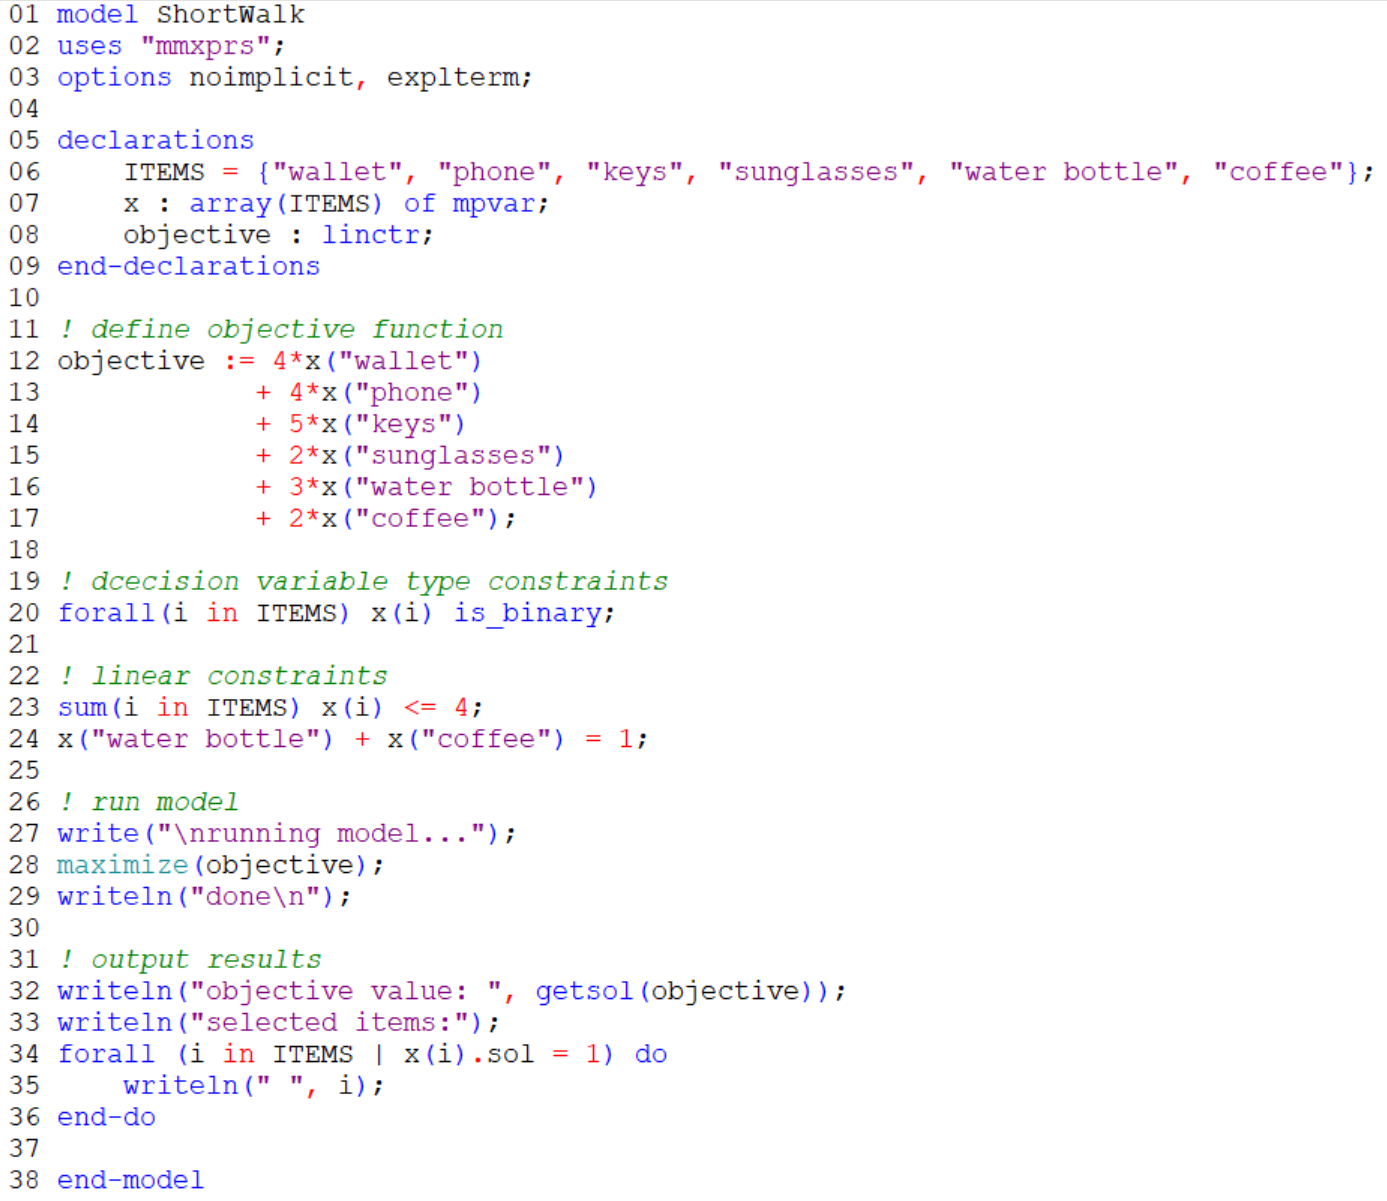
\includegraphics[scale=0.6]{code.png}
            
            \item \textbf{Run the script. Which items were selected? } 
            
            The selected items were: wallet, phone, keys, and water bottle.
            
        \end{enumerate}
    \end{enumerate}
    
    \newpage
    \item
    \begin{enumerate}[A.]
        \item
        \begin{enumerate}[a.]
            \item \textbf{How many sites are there?}
            
            There are eight sites, corresponding to the binary decision variables $X_1, \dots, X_8$.
            
            \item \textbf{What is the objective function? Write this code as an equation.}
            
            The objective function is defined in line 14 as
            \[
                \sum_{i = 1}^8 X_i.
            \]
            
            \item \textbf{What is constraint 1 (\textit{constr1}) doing? Explain in one sentence.}
            
            The first constraint is
            \[
                X_1 + X_2 + X_4 \geq 1,
            \]
            which requires that out of sites 1, 2, and 4, at least one must be selected.
            
            \item \textbf{Is this a minimization or maximization problem? Which line tells you this?}
            
            Line 29 specifies that this is a minimization problem.
            
            \item \textbf{What do lines 33 -- 34 do?}
            
            These lines output the selected sites.
            
            \item \textbf{Run the problem. Which sites were selected?}
            
            Sites 4 and 5 were selected.
        \end{enumerate}
        
        \item Create a thematic map in ArcGIS.
        
        \includegraphics[scale=0.5]{map.png}
        
    \end{enumerate}

\end{enumerate}


\end{document}